%************************************************
\chapter{Assessment of current Business Process Management Solutions}\label{ch:assessment}
%************************************************

The lack of flexibility in handling event subscription in business processes has been outlined in the previous chapters and a set of extended requirements to process management solutions have been presented.
In this section I take a closer look at the capabilities of current solutions with regards to the event occurrence scenarios to get a better understanding of the issues that arise when working with event subscription in business processes.
The assessment will be carried out using BPMN and Camunda, a state-of-the art and widely adopted business process engine.
The main goal is be to identify and illustrate the shortcomings of the current process technology stack. These shortcomings will be referenced in addition to the presented requirements to develop a more refined subscription handling model in the following chapter. \todo[inline]{"subscription handling model"?}

\section{BPMN Models in presence of the Event Occurrence Scenarios}
Chapter X has revealed that processes can run into deadlocks if events do not occur at the right time \todo[inline]{.}
\begin{figure}[]
	\myfloatalign
	{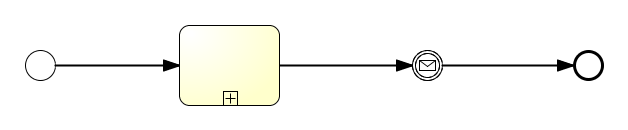
\includegraphics[width=1\linewidth]{chapters/assessment/process-with-intermediate-event.png}}
	\caption{Abstract Process using an Intermediate Catch Event}\label{fig:abstract-process-with-event}
\end{figure}

\autoref{fig:abstract-process-with-event} shows a generalized process that uses an Intermediate Catch Event just before process termination.
In this section I first describe for each Event Occurrence Scenario how this simple event implementation behaves in presence of the given scenario. I then evaluate if it is feasible to create a BPMN model that is free from deadlock in these situations. 

\paragraph{Scenario O1: The event occurs after the enabling of the BPMN event}
\begin{figure}[]
	\myfloatalign
	{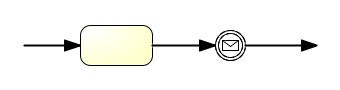
\includegraphics[width=1\linewidth]{chapters/assessment/standard-intermediate-event.png}}
	\caption{Standard Intermediate Catch Event}\label{fig:excerpt-standard-event}
\end{figure}

The first scenario represents the most simple case, that is also natively supported by the BPMN 2.0 specification. When the event occurs after the Event element has been enabled, the event will be received and the process can proceed normally. The use of a standard Intermediate Catch Event does suffice to cover this situation.

\paragraph{Scenario O2: The event does not occur}
\begin{figure}[]
	\myfloatalign
	{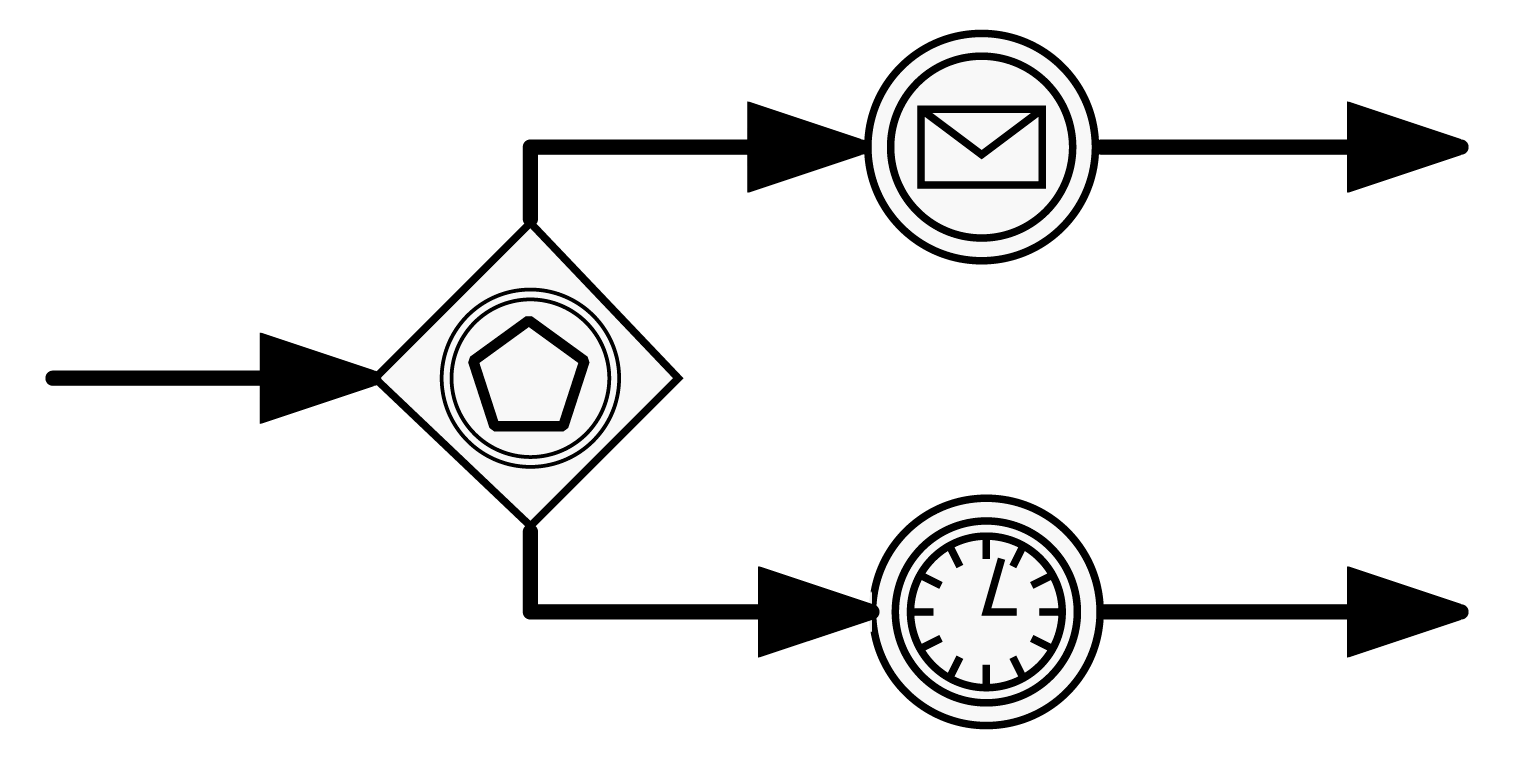
\includegraphics[width=1\linewidth]{chapters/assessment/parallel-timer-event.png}}
	\caption{Intermediate Event with a parallel Timer Event}\label{fig:excerpt-event-with-timer}
\end{figure}

In certain situations an event might not occur at all. Given a basic event implementation like in \autoref{fig:abstract-process-with-event}, the process flow will get to a halt once it reaches the Intermediate Catch Event and not be able to proceed. While depending on the process design this might be the desired behavior, in many situations this is not acceptable.

Let's consider a process that is supposed to wait for approval for a certain amount of time and trigger an additional request if the approval has not been issued before the deadline. \autoref{fig:excerpt-event-with-timer} shows how this behavior can be implemented using an Event-based Gateway which puts a Timer Event in parallel to the Intermediate Catch Event. This extension will make sure that a process does not run into a deadlock state if an expected event does not occur.

\todo[inline]{I mention an example, but that example is not exactly illustrated in the process}
\todo[inline]{according to the spec: what exactly will happen to the active catch event?}


\paragraph{Scenario O3: Between Process instantiation and the enabling of the BPMN event}
\begin{figure}[]
	\myfloatalign
	{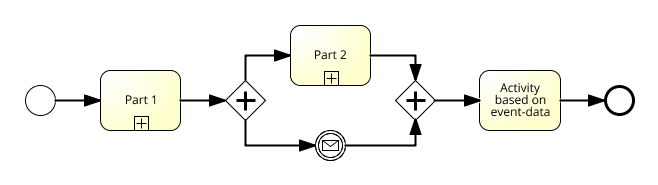
\includegraphics[width=1\linewidth]{chapters/assessment/parallel-gateway-early-subscription.png}}
	\caption{Event Element after Parallel Gateway}\label{fig:excerpt-parallel-gateway-event}
\end{figure}

\todo[inline]{could add a condition "Is data available yet?" to also support the normal occurrence scenario O1}

\paragraph{Scenarios O4 and 05: Before Process Instantiation}
\begin{figure}[]
	\myfloatalign
	{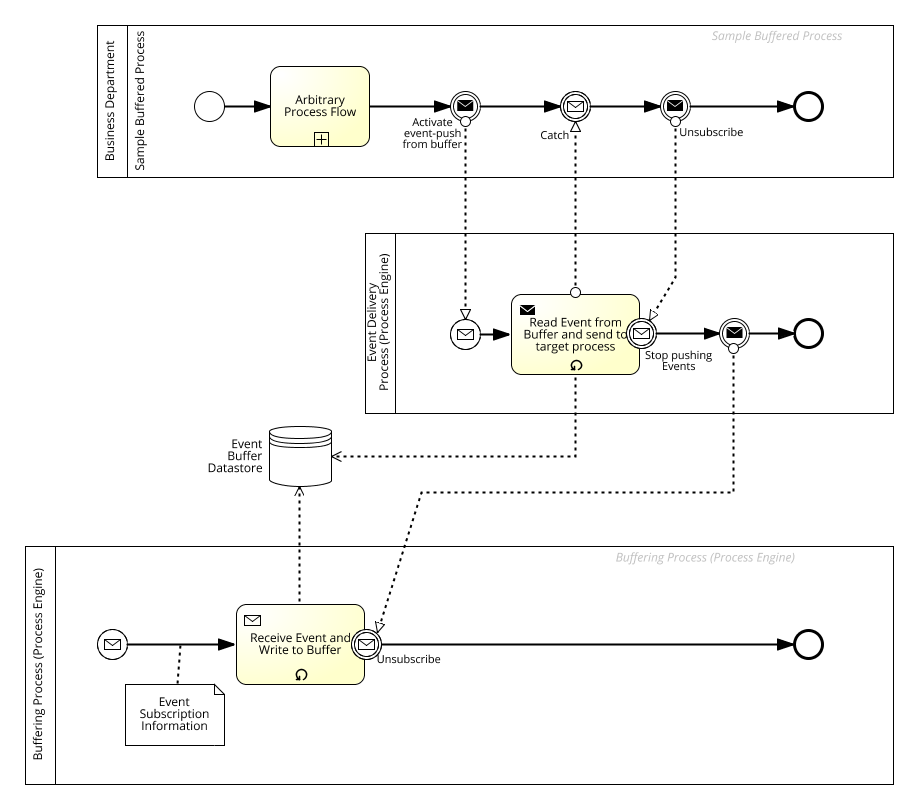
\includegraphics[width=1\linewidth]{chapters/assessment/aux-buffer-process.png}}
	\caption{Event Buffering through an auxiliary Buffering Process}\label{fig:aux-buffering-process}
\end{figure}


\section{Implemention of Early Event Subscription using standard Camunda}
Is it possible to implement this using out-of-the-box Camunda?
Which aspects cannot be (sufficiently) implemented?
How can … be implemented in Camunda? Show details. Diagrams in appendix.
(3 pages)

\section{Discussion}
What are the shortcomings when using out-of-the-box business process solutions to implement
Early Event Subscription?
What can be implemented without problems?
(2 pages)